\subsubsection{Probleme mit mutierenden Problemmengen}
Der erste Ansatz zur Mutation von Problemmengen war - ähnlich der Mutation von Automaten - wie folgt aufgebaut:
\begin{enumerate}
  \item Beim durchgehen und testen der einzelnen Automaten wird gezählt welches Problem wie oft korrekt gelöst wurde
  \item Die Probleme werden nach dem Zähler sortiert 
  \item Die schwierigere hälfte (schlechter gelöst) wird beibehalten
  \item Die einfachere Hälfte wird durch neue zufällige Probleme ersetzt
\end{enumerate}

Dies führte dazu, dass die Problemmenge schneller schwieriger wurde, als die Automaten besser. Warum das zu einem Problem wird ist folgend anhand eines Beispiels erläutert:

Wir haben folgendes Setup:
\begin{itemize}
  \item 200 Automaten als Lösungskandidaten
  \item 1000 Probleme in der Problemmenge
  \item Algorithmus mit globaler, mutierender Problemmenge, welche sich wie oben beschrieben verhält.
\end{itemize}

Der Algorithmus wurde gestartet und es wurden Histogramme der Ergebnisse der Fitnessfunktion der einzelnen Lösungskandidaten erstellt. Die Fitnessfunktion gibt an wieviele der 1000 Probleme der Lösungskandidat richtig gelöst hat.

\begin{figure}[h]
  \centering
  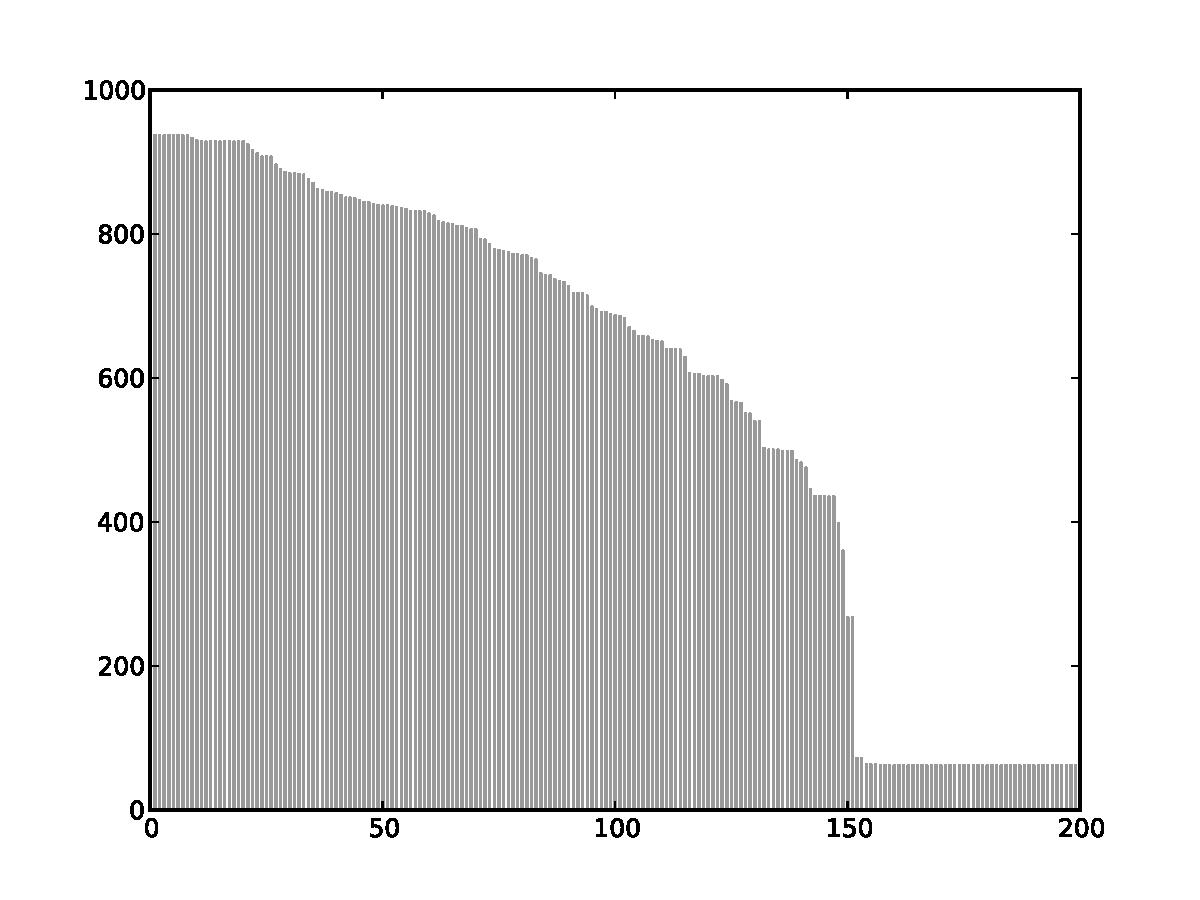
\includegraphics[width=0.8\textwidth]{./images/before_mutation.pdf}
  \caption[Fitnessfunktion der Lösungskandidaten Ausgangslage]{Fitnessfunktion der Lösungskandidaten Ausgangslage}
\end{figure}

Beim ersten Histogramm sieht man den Wert der Fitnessfunktion von 200 zufällig generierte Automaten welche versuchen 1000 zufällig generierte Probleme zu lösen. Einige Automaten schneiden besser ab, einige schlechter. Aber die Verteilung ist zufällig. 

\begin{figure}[h]
  \centering
  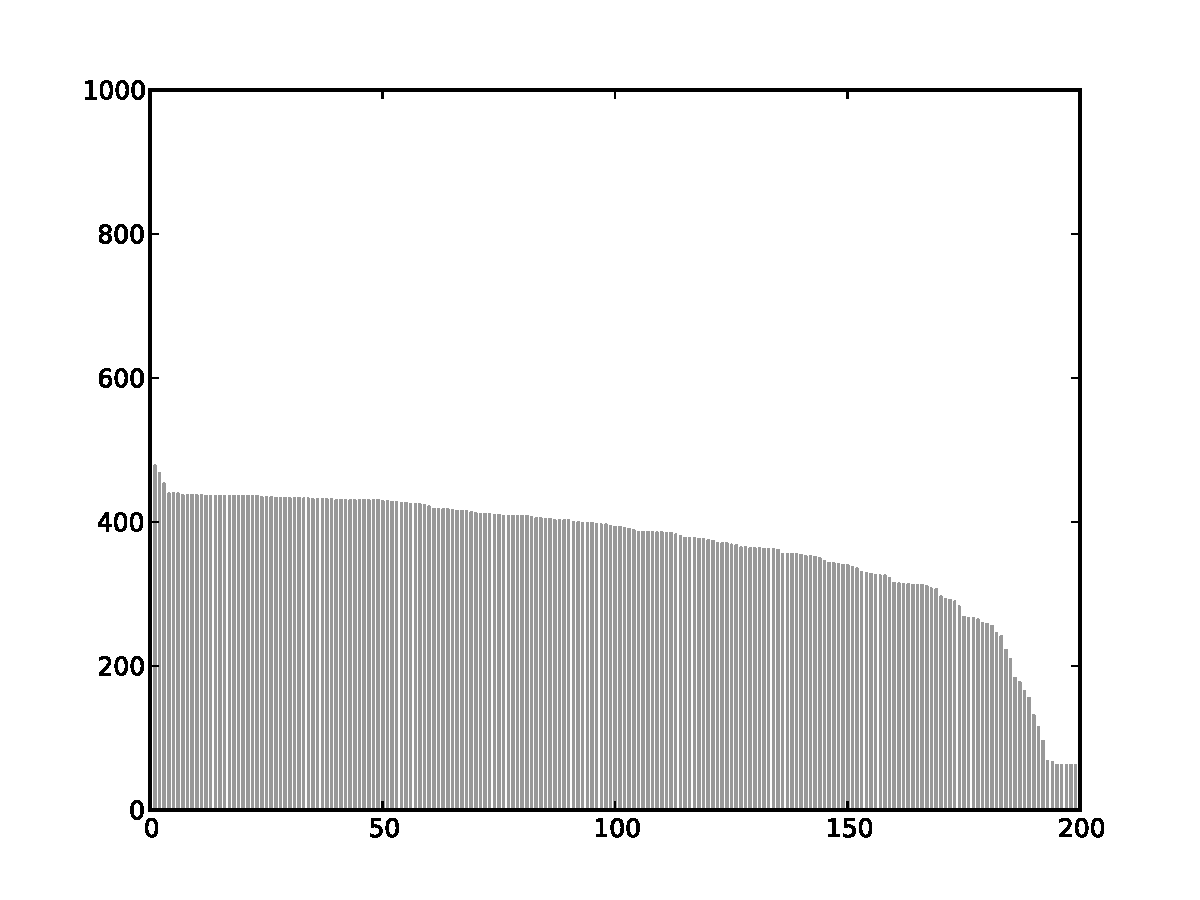
\includegraphics[width=0.8\textwidth]{./images/one_iteration.pdf}
  \caption[Fitnessfunktion der Lösungskandidaten nach einer Iteration]{Fitnessfunktion der Lösungskandidaten nach einer Iteration}
\end{figure}

Nach einer Iteration lösen unsere Automaten das Ganze schon viel schlechter. Das liegt daran, dass die 500 leichtesten Probleme mit grosser Wahrscheinlichkeit von einem Grossteil der besseren Automaten gelöst werden konnten und eben diese Probleme wurden nun entfernt und durch neue, tendenziell schwierigere Probleme ersetzt. Die Automaten hingegen können sich in einer Iteration kaum verbessern.

\begin{figure}[h]
  \centering
  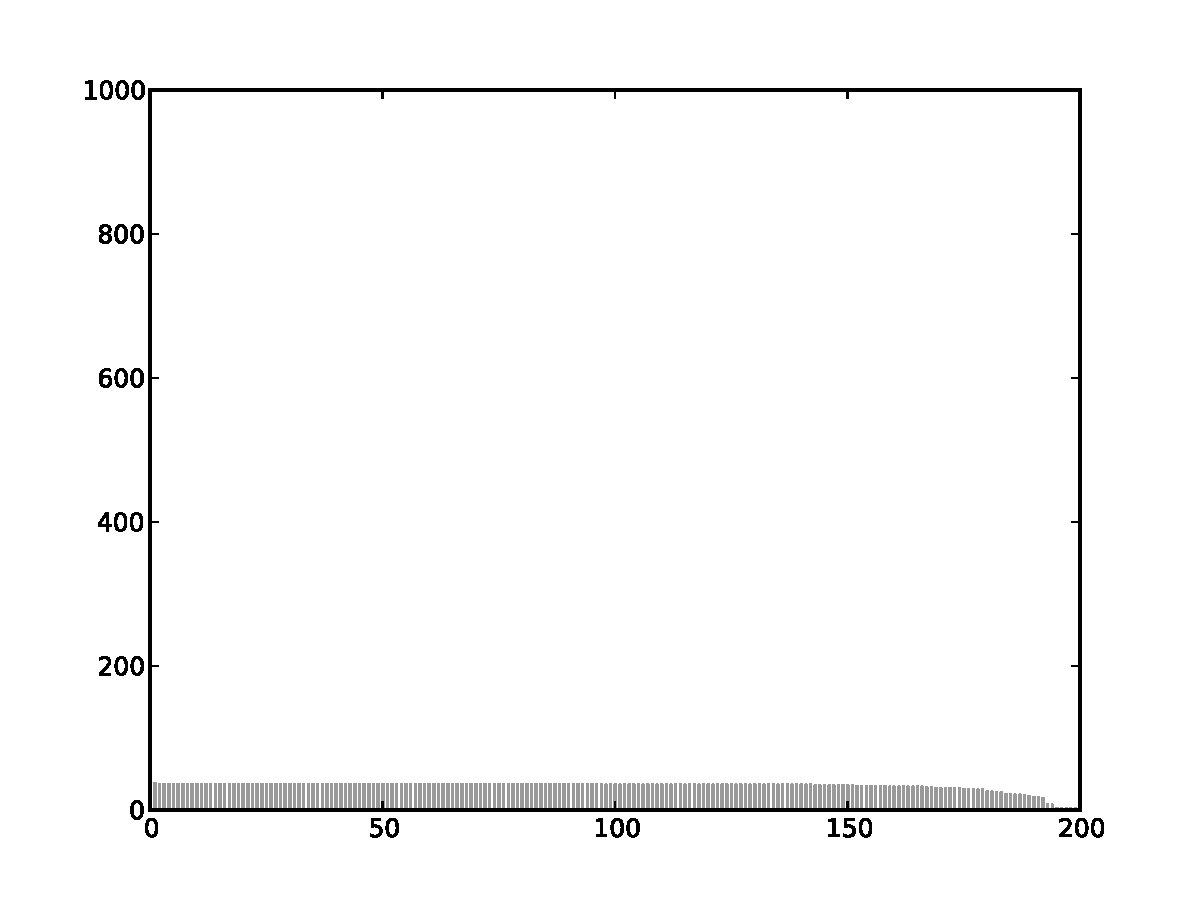
\includegraphics[width=0.8\textwidth]{./images/fife_iterations.pdf}
  \caption[Fitnessfunktion der Lösungskandidaten nach fünf Iterationen]{Fitnessfunktion der Lösungskandidaten nach fünf Iterationen}
\end{figure}

Nach fünf Iterationen sieht man wozu das Ganze führt: Die Probleme sind nun so schwierig, dass um 95\% der Probleme von keinem unserer Automaten mehr gelöst werden kann. Dies führt dazu, dass keine Unterschiede zwischen guten und schlechten Automaten mehr feststellbar sind was wiederum dazu führt, dass der Algorithmus nicht konvergiert.